\documentclass[11pt]{article}
\usepackage[margin=1cm,papersize={22cm,30cm}]{geometry}
\usepackage{amsmath,amssymb,bm,tikz}
\usetikzlibrary{calc,arrows.meta,positioning}
\usepackage{hyperref}
\newcommand{\cref}[1]{[ref]}
%%%%%%%%%%%%%%%%%%%%%%%%%%%%%%%%%%%%%%%%%
% Mathematics Macros and Commands
% Custom mathematical notation and shortcuts
%%%%%%%%%%%%%%%%%%%%%%%%%%%%%%%%%%%%%%%%%

%----------------------------------------------------------------------------------------
%	Formatting
%----------------------------------------------------------------------------------------

%----------------------------------------------------------------------------------------
%	MATHEMATICAL OPERATORS AND SYMBOLS
%----------------------------------------------------------------------------------------

%  Expected value operator
\DeclareMathOperator{\E}{\mathbb{E}}

% Mean opertations
\DeclareMathOperator{\Moy}{\operatorname{Moy}}

% Covariance operator
\DeclareMathOperator{\Var}{\operatorname{Var}}
\DeclareMathOperator{\Cov}{\operatorname{Cov}}

%  Probability operator (using different name to avoid conflict)
\DeclareMathOperator{\Prob}{\mathbb{P}}
\DeclareMathOperator{\Tr}{\operatorname{Tr}} %  Trace

\newcommand{\T}{\mathrm{T}} % Transpose
\newcommand{\herm}{\mathrm{H}} % Conjugate (hermitian) transpose
\newcommand{\conj}[1]{{#1}^{*}} % Complex conjugate
\DeclareMathOperator{\Realp}{\operatorname{Re}} % Real part
\DeclareMathOperator{\Imagp}{\operatorname{Im}} % Imaginary part
\DeclareMathOperator{\Diag}{\operatorname{diag}} % Determinant
\DeclareMathOperator{\Cond}{k} % Condition number


\newcommand{\diff}{\mathrm{d}} % Differential
\DeclareMathOperator{\Det}{\operatorname{det}} % Determinant

% Linear algebra
\newcommand{\inv}[1]{{#1}^{-1}}
\newcommand{\quadratic}[2]{#1^\T \inv{#2} #1 }
\newcommand{\quadraticH}[2]{#1^\herm \inv{#2} #1 } % Hermitian quadratic form
\newcommand{\q}[2]{\mathcal{q}\left(#1, #2\right)}
\newcommand{\eqdef}{\triangleq} % Definition equality
\newcommand{\intrange}[2]{\{#1,\dots,#2\}} % Integer range


%----------------------------------------------------------------------------------------
%	MATHEMATICAL SHORTCUTS
%----------------------------------------------------------------------------------------

%  Real numbers set
\newcommand{\R}{\mathbb{R}}
\newcommand{\C}{\mathbb{C}}

%  Natural numbers set
\newcommand{\N}{\mathbb{N}}

%  Norm notation
\newcommand{\norm}[1]{\left\lVert#1\right\rVert}

%  Absolute value
\newcommand{\abs}[1]{\left\lvert#1\right\rvert}

%  Trace
\newcommand{\trace}[1]{\Tr\left\{#1\right\}}


% Hypothesis testing
\newcommand{\detect}{\;\underset{\hypothesis_0}{\overset{\hypothesis_1}{\gtrless}}\; \DetectorTreshold}


%----------------------------------------------------------------------------------------
%	MATHEMATICAL FORMATTING
%----------------------------------------------------------------------------------------
%  Matrix notation shortcut
\newcommand{\mat}[1]{\boldsymbol{#1}}

%  Vector notation shortcut (renaming to avoid conflict)
\renewcommand{\vector}[1]{\boldsymbol{#1}}



%----------------------------------------------------------------------------------------
%	Computer science
%----------------------------------------------------------------------------------------
\newcommand{\bigO}{\mathcal{O}}


%%%%%%%%%%%%%%%%%%%%%%%%%%%%%%%%%%%%%%%%%
%	COMMON DEFINITIONS IN THIS HDR DISSERTATION
%----------------------------------------------------------------------------------------


%----------------------------------------------------------------------------------------
% Vectors and matrix dimensions
%----------------------------------------------------------------------------------------
\newcommand{\vdim}{d}
\newcommand{\matrixdimR}{M}
\newcommand{\matrixdimC}{N}

%----------------------------------------------------------------------------------------
% Linear algebra
%----------------------------------------------------------------------------------------
\newcommand{\Id}[1]{\mat{I}_{#1}} % Identity matrix of given dimension
\newcommand{\Orth}{\mat{O}} % Orthogonal matrix
\newcommand{\eig}{\lambda} % Eigenvalues
\newcommand{\eigset}{\Lambda} % Eigenvalues set
\newcommand{\frob}{\mathbb{F}} % Frobenius norm text
\newcommand{\SPD}[1]{\mathcal{S}_{#1}^{++}} % Set of SPD matrices of given dimension
\newcommand{\HPD}[1]{\mathcal{H}_{#1}^{++}} % Set of hermitian positive definite matrices
\newcommand{\complexform}[1]{\mathcal{M}\left(#1\right)} % Real form of a complex matrix
\newcommand{\Unit}{\mat{U}} % Unitary matrix

%----------------------------------------------------------------------------------------
% Statistics
%----------------------------------------------------------------------------------------
\newcommand{\Variable}{\mathcal{X}} % underlying random variable. multivariate case
\newcommand{\Variablebis}{\mathcal{Y}} % underlying random variable bis. multivariate case
\newcommand{\variable}{X} % underlying random variable
\newcommand{\variablebis}{X} % underlying random variable bis
\newcommand{\x}{\vector{x}} % observed sample
\newcommand{\y}{\vector{y}} % observed sample two
\newcommand{\X}{\mat{X}} % observed data as a matrix : all samples
\newcommand{\Xset}{\mathfrak{X}} % observed data as a set : all samples
\newcommand{\moy}{\mu} % mean of a random variable
\newcommand{\Vmoy}{\mat{\moy}} % mean of a random variable. multivariate case
\newcommand{\var}{\sigma^2} % variance of a random variable
\newcommand{\std}{\sigma} % Standard deviation
\newcommand{\texture}{\tau} % texture parameter
\newcommand{\MCov}{\mat{\Sigma}} % Covariance matrix
\newcommand{\MPCov}{\mat{C}} % Pseudo-covariance (relation) matrix
\newcommand{\MErr}{\mat{P}} % Error matrix of the widely linear predictor
\newcommand{\MWl}{\mat{R}} % Widely linear predictor matrix
\newcommand{\Nobs}{N}
\newcommand{\Ntime}{T} % Number of time values in a temporal scenario
\newcommand{\Nvar}{\vdim} % number of varaibles
\newcommand{\Niter}{n_{\mathrm{iter}}} % Number of iterations of an algorithm
\newcommand{\ivar}{i} % index on variables
\newcommand{\ivarbis}{j} % index on variables bis
\newcommand{\iobs}{k} % index on observations
\newcommand{\igroup}{t} % index on group of observations
\newcommand{\itime}{t} % time index
\newcommand{\coefledoitwolf}{\alpha} % LedoitWolf estimator coef
\newcommand{\targetledoitwolf}{\mat{T}} % LedoitWolf estimator target matrix
\newcommand{\hypothesis}{\mathcal{H}} % Hypothesis in a Neyman-Pearson scheme
\newcommand{\statistic}{\Lambda} % Some statistic over the data
\newcommand{\DetectorStat}{\hat{\statistic}} % Some test statistic of a Neyman-Pearson problem
\newcommand{\DetectorTreshold}{\lambda} % Detector tresholding value
\newcommand{\Smat}{\mathbf{S}} % Sum of X@X.T
\newcommand{\Tyler}{\widehat{\bm{\mathcal{T}}}} % Tyler estimator

%----------------------------------------------------------------------------------------
% Probabilities
%----------------------------------------------------------------------------------------
\newcommand{\p}[1]{p_{#1}} % legacy for ddp
\newcommand{\ddp}[1]{f_{#1}}
\newcommand{\Universe}{\Omega} % Univers en proba
\newcommand{\event}{\omega} % Evenement élémentaire
\newcommand{\param}{\theta} % Unspecified probability parameter
\newcommand{\gaussian}{\mathcal{N}} % Gaussian distribution
\newcommand{\compoundgaussian}{\mathcal{CG}} % Compound-Gaussian distribuion
\newcommand{\elliptical}{\mathcal{E}} % Elliptical distribution
\newcommand{\angular}{\mathcal{AE}} % Angular elliptical distribution
\newcommand{\studentdist}{\mathcal{T}} % t-distribution
\newcommand{\kdist}{\mathcal{K}} % K-distribution
\newcommand{\gengaussian}{\mathcal{GG}} % Generalized Gaussian distribution
\newcommand{\gammadist}{\mathcal{G}} % Gamma distribution
\newcommand{\chisquared}{\chi^2} % Chi-squared distribution
\newcommand{\uniform}{\mathcal{U}} % Uniform distribution
\newcommand{\wishart}{\mathcal{W}} % Wishart distribution
\newcommand{\cgaussian}{\mathcal{CN}} % Complex circular Gaussian distribution
\newcommand{\celliptical}{\mathcal{CE}} % Complex elliptical distribution
\newcommand{\ccompoundgaussian}{\mathcal{CCG}} % Complex compound-Gaussian distribution
\newcommand{\cwishart}{\mathcal{CW}} % Complex Wishart distribution
\newcommand{\cangular}{\mathcal{CAG}} % Complex angular central Gaussian distribution
\newcommand{\gcgaussian}{\mathcal{GCN}} % Generalised (non-circular) complex Gaussian
\newcommand{\likelihood}{\ell} % Log-likelihood function

%----------------------------------------------------------------------------------------
% Elliptical distributions
%----------------------------------------------------------------------------------------
\newcommand{\densgen}{g} % Density generator of an elliptical distribution
\newcommand{\densgenmoment}[1]{\mathfrak{m}_{#1,\densgen}} % Finite moment of the density generator
\newcommand{\densgenconst}[1]{\mathfrak{c}_{#1,\densgen}} % Normalisation constant of the d.d.p
\newcommand{\densgenmomentC}[1]{\tilde{\mathfrak{m}}_{#1,\densgen}} % Finite moment, complex case
\newcommand{\densgenconstC}[1]{\tilde{\mathfrak{c}}_{#1,\densgen}} % Normalisation constant, complex case
\newcommand{\sphere}[1]{\mathbb{S}^{#1}} % Unit sphere
\newcommand{\csphere}[1]{\mathbb{CS}^{#1}} % Complex unit sphere
\newcommand{\spherearea}[1]{\mathfrak{s}_{#1}} % Surface area of the unit sphere
\newcommand{\modvar}{\mathcal{R}} % Modular variate
\newcommand{\quadvar}{\mathcal{Q}} % Quadratic form random variable
\newcommand{\dof}{\nu} % Degrees of freedom / texture shape parameter
\newcommand{\MScatter}{\mat{S}} % Scatter matrix
\newcommand{\MShape}{\mat{\xi}} % Shape matrix

%----------------------------------------------------------------------------------------
% Robust estimation
%----------------------------------------------------------------------------------------
\newcommand{\weight}{u} % Weight function of an M-estimator
\newcommand{\Mestim}{\tilde{\MScatter}} % M-estimator of scatter
\newcommand{\iiter}{n} % Index on the iterations of an algorithm
\DeclareMathOperator{\vecop}{vec} % Vectorisation operator
\newcommand{\Kmat}{\mat{K}} % Commutation matrix
\newcommand{\scorefun}{\psi} % psi(t) = t u(t)


%----------------------------------------------------------------------------------------
% Optimization
%----------------------------------------------------------------------------------------
\newcommand{\loss}{\mathcal{L}} % Loss function
\newcommand{\risk}{\mathcal{R}} % Expected risk function
\newcommand{\opt}{\star} % Optimal point


%----------------------------------------------------------------------------------------
% Remote Sensing
%----------------------------------------------------------------------------------------
\newcommand{\HH}{\mathrm{HH}}
\newcommand{\VH}{\mathrm{VH}}
\newcommand{\HV}{\mathrm{HV}}
\newcommand{\VV}{\mathrm{VV}}




\pagestyle{empty}
\begin{document}
\centering
% Variete, courbe tracee dessus, et espace tangent en un point.
% Utilise dans la \cref{sec:context-riemann-notion}.
% Styles et briques communs aux figures de geometrie riemannienne du
% \cref{ch:context-riemann}. Ce fichier peut etre \input plusieurs fois.
\definecolor{rmanifold}{RGB}{90,90,90}
\definecolor{rtangent}{RGB}{50,110,120}
\definecolor{rgeodesic}{RGB}{40,70,140}
\definecolor{rvector}{RGB}{175,95,45}
\tikzset{
  riemann/.style={
    >={Stealth[length=4.5pt,width=3.5pt]},
    line join=round,
    font=\footnotesize,
  },
  % La nappe qui represente la variete, centree sur l'origine.
  rsurface/.pic={
    \fill[rmanifold!7]
      (-3.2,0.15) .. controls (-2.95,1.75) and (-1.5,2.35) .. (0,2.35)
      .. controls (1.5,2.35) and (2.95,1.7) .. (3.2,0.15)
      .. controls (1.9,-0.7) and (-1.9,-0.7) .. (-3.2,0.15) -- cycle;
    \draw[rmanifold!70, thick]
      (-3.2,0.15) .. controls (-2.95,1.75) and (-1.5,2.35) .. (0,2.35)
      .. controls (1.5,2.35) and (2.95,1.7) .. (3.2,0.15);
    \draw[rmanifold!70, thick]
      (-3.2,0.15) .. controls (-1.9,-0.7) and (1.9,-0.7) .. (3.2,0.15);
  },
  % Le plan tangent, a placer en un point donne via un shift.
  rplane/.pic={
    \fill[rtangent!10, draw=rtangent!65]
      (-1.35,-0.42) -- (1.55,-0.88) -- (2.05,0.22) -- (-0.85,0.68) -- cycle;
  },
}

\begin{tikzpicture}[riemann]
  \coordinate (P) at (-1.04,1.38);

  \path (0,0) pic {rsurface};
  \node[rmanifold!85] at (2.55,1.55) {$\Manifold$};

  % plan tangent
  \path (P) pic[scale=0.85] {rplane};
  \node[rtangent!90, anchor=east, inner sep=1pt] at ($(P)+(-1.20,0.50)$)
    {$\Tangent{\param}{\Manifold}$};

  % courbe tracee sur la variete
  \draw[rgeodesic, very thick]
    (-2.6,0.85) .. controls (-2.0,1.30) and (-0.2,1.55) .. (0.9,1.62);
  \node[rgeodesic, anchor=south west, inner sep=1pt] at (0.72,1.62) {$\geod$};

  % vitesse : un vecteur tangent
  \draw[rvector, very thick, ->] (P) -- ($(P)+(1.20,0.15)$);
  \node[rvector, anchor=north west, inner sep=1pt] at ($(P)+(0.55,0.10)$)
    {$\dot{\geod}(0)$};

  \fill (P) circle (1.7pt);
  \node[anchor=south east, inner sep=2pt] at (P) {$\param$};
\end{tikzpicture}
\par\vspace{1cm}
% La metrique : produit scalaire sur l'espace tangent, donc norme et angle,
% et par integration longueur d'une courbe.
% Utilise dans la \cref{sec:context-riemann-notion}.
% Styles et briques communs aux figures de geometrie riemannienne du
% \cref{ch:context-riemann}. Ce fichier peut etre \input plusieurs fois.
\definecolor{rmanifold}{RGB}{90,90,90}
\definecolor{rtangent}{RGB}{50,110,120}
\definecolor{rgeodesic}{RGB}{40,70,140}
\definecolor{rvector}{RGB}{175,95,45}
\tikzset{
  riemann/.style={
    >={Stealth[length=4.5pt,width=3.5pt]},
    line join=round,
    font=\footnotesize,
  },
  % La nappe qui represente la variete, centree sur l'origine.
  rsurface/.pic={
    \fill[rmanifold!7]
      (-3.2,0.15) .. controls (-2.95,1.75) and (-1.5,2.35) .. (0,2.35)
      .. controls (1.5,2.35) and (2.95,1.7) .. (3.2,0.15)
      .. controls (1.9,-0.7) and (-1.9,-0.7) .. (-3.2,0.15) -- cycle;
    \draw[rmanifold!70, thick]
      (-3.2,0.15) .. controls (-2.95,1.75) and (-1.5,2.35) .. (0,2.35)
      .. controls (1.5,2.35) and (2.95,1.7) .. (3.2,0.15);
    \draw[rmanifold!70, thick]
      (-3.2,0.15) .. controls (-1.9,-0.7) and (1.9,-0.7) .. (3.2,0.15);
  },
  % Le plan tangent, a placer en un point donne via un shift.
  rplane/.pic={
    \fill[rtangent!10, draw=rtangent!65]
      (-1.35,-0.42) -- (1.55,-0.88) -- (2.05,0.22) -- (-0.85,0.68) -- cycle;
  },
}

\begin{tikzpicture}[riemann]
  \coordinate (P) at (-1.70,1.15);

  \path (0,0) pic {rsurface};
  \node[rmanifold!85] at (2.85,1.15) {$\Manifold$};

  % plan tangent et deux vecteurs
  \path (P) pic[scale=0.75] {rplane};
  \draw[rvector, very thick, ->] (P) -- ($(P)+(1.10,-0.16)$);
  \node[rvector, anchor=north west, inner sep=1pt] at ($(P)+(0.85,-0.14)$) {$\tvec$};
  \draw[rvector, very thick, ->] (P) -- ($(P)+(0.40,0.46)$);
  \node[rvector, anchor=south east, inner sep=1pt] at ($(P)+(0.42,0.44)$) {$\tvecbis$};
  \draw[rtangent!80] ($(P)+(0.46,-0.07)$) arc[start angle=-8, end angle=48, radius=0.47];
  \node[rtangent!90, font=\scriptsize, anchor=west] at ($(P)+(0.80,0.42)$)
    {$\metric{\tvec}{\tvecbis}{\param}$};
  \node[rtangent!90, anchor=north, inner sep=2pt] at ($(P)+(0.10,-0.50)$)
    {$\Tangent{\param}{\Manifold}$};

  % longueur d'une courbe : vitesses echantillonnees le long du chemin
  \draw[rgeodesic, very thick]
    (0.55,1.85) .. controls (1.45,1.95) and (2.05,1.55) .. (2.45,0.95);
  \node[rgeodesic, anchor=south east, inner sep=1pt] at (0.60,1.88) {$\geod$};
  \foreach \x/\y/\dx/\dy in {0.85/1.91/0.30/0.05, 1.60/1.89/0.28/-0.13, 2.22/1.42/0.18/-0.28}
    \draw[rvector!85, thick, ->] (\x,\y) -- ++(\dx,\dy);
  \node[rgeodesic!85, anchor=north, font=\scriptsize] at (1.35,1.32)
    {$L(\geod)=\int\normriem{\dot{\geod}}{\geod}$};

  \fill (P) circle (1.7pt);
  \node[anchor=south east, inner sep=2pt] at (P) {$\param$};
\end{tikzpicture}
\par\vspace{1cm}
% Projection orthogonale d'un vecteur de l'espace ambiant sur l'espace tangent.
% Utilise dans la \cref{sec:context-riemann-notion}.
% Styles et briques communs aux figures de geometrie riemannienne du
% \cref{ch:context-riemann}. Ce fichier peut etre \input plusieurs fois.
\definecolor{rmanifold}{RGB}{90,90,90}
\definecolor{rtangent}{RGB}{50,110,120}
\definecolor{rgeodesic}{RGB}{40,70,140}
\definecolor{rvector}{RGB}{175,95,45}
\tikzset{
  riemann/.style={
    >={Stealth[length=4.5pt,width=3.5pt]},
    line join=round,
    font=\footnotesize,
  },
  % La nappe qui represente la variete, centree sur l'origine.
  rsurface/.pic={
    \fill[rmanifold!7]
      (-3.2,0.15) .. controls (-2.95,1.75) and (-1.5,2.35) .. (0,2.35)
      .. controls (1.5,2.35) and (2.95,1.7) .. (3.2,0.15)
      .. controls (1.9,-0.7) and (-1.9,-0.7) .. (-3.2,0.15) -- cycle;
    \draw[rmanifold!70, thick]
      (-3.2,0.15) .. controls (-2.95,1.75) and (-1.5,2.35) .. (0,2.35)
      .. controls (1.5,2.35) and (2.95,1.7) .. (3.2,0.15);
    \draw[rmanifold!70, thick]
      (-3.2,0.15) .. controls (-1.9,-0.7) and (1.9,-0.7) .. (3.2,0.15);
  },
  % Le plan tangent, a placer en un point donne via un shift.
  rplane/.pic={
    \fill[rtangent!10, draw=rtangent!65]
      (-1.35,-0.42) -- (1.55,-0.88) -- (2.05,0.22) -- (-0.85,0.68) -- cycle;
  },
}

\begin{tikzpicture}[riemann]
  \coordinate (P) at (-0.45,1.35);

  \path (0,0) pic {rsurface};
  \node[rmanifold!85] at (2.55,1.80) {$\Manifold$};

  \path (P) pic {rplane};
  \node[rtangent!90, anchor=east] at ($(P)+(-1.30,0.50)$)
    {$\Tangent{\param}{\Manifold}$};

  % vecteur ambiant, hors du plan tangent
  \draw[rmanifold!85, very thick, ->] (P) -- ($(P)+(1.10,1.15)$);
  \node[rmanifold, anchor=south west, inner sep=1pt] at ($(P)+(1.08,1.13)$)
    {$\mat{Z}\in\ambient$};

  % sa projection
  \draw[rvector, very thick, ->] (P) -- ($(P)+(1.32,-0.18)$);
  \node[rvector, anchor=north, inner sep=2pt] at ($(P)+(1.05,-0.22)$)
    {$\projman_{\param}(\mat{Z})$};

  % trait de projection
  \draw[rmanifold!60, dashed] ($(P)+(1.10,1.15)$) -- ($(P)+(1.32,-0.18)$);

  \fill (P) circle (1.7pt);
  \node[anchor=north east, inner sep=2pt] at (P) {$\param$};
\end{tikzpicture}
\par\vspace{1cm}
% Geodesique entre deux points et distance geodesique, comparees a une autre
% courbe tracee sur la variete.
% Utilise dans la \cref{sec:context-riemann-notion}.
% Styles et briques communs aux figures de geometrie riemannienne du
% \cref{ch:context-riemann}. Ce fichier peut etre \input plusieurs fois.
\definecolor{rmanifold}{RGB}{90,90,90}
\definecolor{rtangent}{RGB}{50,110,120}
\definecolor{rgeodesic}{RGB}{40,70,140}
\definecolor{rvector}{RGB}{175,95,45}
\tikzset{
  riemann/.style={
    >={Stealth[length=4.5pt,width=3.5pt]},
    line join=round,
    font=\footnotesize,
  },
  % La nappe qui represente la variete, centree sur l'origine.
  rsurface/.pic={
    \fill[rmanifold!7]
      (-3.2,0.15) .. controls (-2.95,1.75) and (-1.5,2.35) .. (0,2.35)
      .. controls (1.5,2.35) and (2.95,1.7) .. (3.2,0.15)
      .. controls (1.9,-0.7) and (-1.9,-0.7) .. (-3.2,0.15) -- cycle;
    \draw[rmanifold!70, thick]
      (-3.2,0.15) .. controls (-2.95,1.75) and (-1.5,2.35) .. (0,2.35)
      .. controls (1.5,2.35) and (2.95,1.7) .. (3.2,0.15);
    \draw[rmanifold!70, thick]
      (-3.2,0.15) .. controls (-1.9,-0.7) and (1.9,-0.7) .. (3.2,0.15);
  },
  % Le plan tangent, a placer en un point donne via un shift.
  rplane/.pic={
    \fill[rtangent!10, draw=rtangent!65]
      (-1.35,-0.42) -- (1.55,-0.88) -- (2.05,0.22) -- (-0.85,0.68) -- cycle;
  },
}

\begin{tikzpicture}[riemann]
  \coordinate (P) at (-1.95,1.05);
  \coordinate (Q) at ( 1.85,1.35);

  \path (0,0) pic {rsurface};
  \node[rmanifold!85] at (2.65,0.55) {$\Manifold$};

  % une courbe quelconque joignant les deux points
  \draw[rmanifold!60, thick, dashed]
    (P) .. controls (-1.20,-0.15) and (1.05,-0.05) .. (Q);
  \node[rmanifold, anchor=north, font=\scriptsize] at (-0.15,0.05)
    {$L(\geod')>\geodist(\param_0,\param_1)$};

  % la geodesique
  \draw[rgeodesic, very thick]
    (P) .. controls (-0.85,2.05) and (0.75,2.15) .. (Q);
  \node[rgeodesic, anchor=east, inner sep=3pt] at (-1.35,1.72) {$\geod$};
  \node[rgeodesic!85, anchor=south, font=\scriptsize] at (0.05,2.06)
    {$L(\geod)=\geodist(\param_0,\param_1)$};

  \fill (P) circle (1.7pt);
  \node[anchor=east, inner sep=3pt] at (P) {$\param_0$};
  \fill (Q) circle (1.7pt);
  \node[anchor=west, inner sep=3pt] at (Q) {$\param_1$};
\end{tikzpicture}
\par\vspace{1cm}
% Applications exponentielle et logarithme riemanniennes.
% Utilise dans la \cref{sec:context-riemann-notion}.
% Styles et briques communs aux figures de geometrie riemannienne du
% \cref{ch:context-riemann}. Ce fichier peut etre \input plusieurs fois.
\definecolor{rmanifold}{RGB}{90,90,90}
\definecolor{rtangent}{RGB}{50,110,120}
\definecolor{rgeodesic}{RGB}{40,70,140}
\definecolor{rvector}{RGB}{175,95,45}
\tikzset{
  riemann/.style={
    >={Stealth[length=4.5pt,width=3.5pt]},
    line join=round,
    font=\footnotesize,
  },
  % La nappe qui represente la variete, centree sur l'origine.
  rsurface/.pic={
    \fill[rmanifold!7]
      (-3.2,0.15) .. controls (-2.95,1.75) and (-1.5,2.35) .. (0,2.35)
      .. controls (1.5,2.35) and (2.95,1.7) .. (3.2,0.15)
      .. controls (1.9,-0.7) and (-1.9,-0.7) .. (-3.2,0.15) -- cycle;
    \draw[rmanifold!70, thick]
      (-3.2,0.15) .. controls (-2.95,1.75) and (-1.5,2.35) .. (0,2.35)
      .. controls (1.5,2.35) and (2.95,1.7) .. (3.2,0.15);
    \draw[rmanifold!70, thick]
      (-3.2,0.15) .. controls (-1.9,-0.7) and (1.9,-0.7) .. (3.2,0.15);
  },
  % Le plan tangent, a placer en un point donne via un shift.
  rplane/.pic={
    \fill[rtangent!10, draw=rtangent!65]
      (-1.35,-0.42) -- (1.55,-0.88) -- (2.05,0.22) -- (-0.85,0.68) -- cycle;
  },
}

\begin{tikzpicture}[riemann]
  \coordinate (P) at (-1.55,1.20);
  \coordinate (Q) at ( 1.75,1.45);

  \path (0,0) pic {rsurface};
  \node[rmanifold!85] at (2.75,0.75) {$\Manifold$};

  \path (P) pic[scale=0.8] {rplane};
  \node[rtangent!90, anchor=east, inner sep=1pt] at ($(P)+(-1.15,0.40)$)
    {$\Tangent{\param_0}{\Manifold}$};

  % la geodesique
  \draw[rgeodesic, very thick]
    (P) .. controls (-0.55,2.10) and (0.75,2.20) .. (Q);

  % le vecteur tangent
  \draw[rvector, very thick, ->] (P) -- ($(P)+(1.60,-0.23)$);
  \node[rvector, anchor=north, inner sep=2pt] at ($(P)+(0.80,-0.34)$)
    {$\tvec=\log_{\param_0}(\param_1)$};

  % le retour sur la variete
  \draw[rvector!60, dotted, very thick, ->]
    ($(P)+(1.63,-0.21)$) .. controls (0.75,0.55) and (1.60,0.70) .. ($(Q)+(0.02,-0.12)$);
  \node[rvector!85, anchor=north, inner sep=2pt, font=\scriptsize] at (1.05,0.62)
    {$\exp_{\param_0}(\tvec)$};

  \fill (P) circle (1.7pt);
  \node[anchor=east, inner sep=3pt] at (P) {$\param_0$};
  \fill (Q) circle (1.7pt);
  \node[anchor=west, inner sep=3pt] at (Q) {$\param_1$};
\end{tikzpicture}
\par\vspace{1cm}
% Transport parallele : deux vecteurs tangents deplaces le long d'une
% geodesique, l'angle qu'ils forment etant conserve.
% Utilise dans la \cref{sec:context-riemann-notion}.
% Styles et briques communs aux figures de geometrie riemannienne du
% \cref{ch:context-riemann}. Ce fichier peut etre \input plusieurs fois.
\definecolor{rmanifold}{RGB}{90,90,90}
\definecolor{rtangent}{RGB}{50,110,120}
\definecolor{rgeodesic}{RGB}{40,70,140}
\definecolor{rvector}{RGB}{175,95,45}
\tikzset{
  riemann/.style={
    >={Stealth[length=4.5pt,width=3.5pt]},
    line join=round,
    font=\footnotesize,
  },
  % La nappe qui represente la variete, centree sur l'origine.
  rsurface/.pic={
    \fill[rmanifold!7]
      (-3.2,0.15) .. controls (-2.95,1.75) and (-1.5,2.35) .. (0,2.35)
      .. controls (1.5,2.35) and (2.95,1.7) .. (3.2,0.15)
      .. controls (1.9,-0.7) and (-1.9,-0.7) .. (-3.2,0.15) -- cycle;
    \draw[rmanifold!70, thick]
      (-3.2,0.15) .. controls (-2.95,1.75) and (-1.5,2.35) .. (0,2.35)
      .. controls (1.5,2.35) and (2.95,1.7) .. (3.2,0.15);
    \draw[rmanifold!70, thick]
      (-3.2,0.15) .. controls (-1.9,-0.7) and (1.9,-0.7) .. (3.2,0.15);
  },
  % Le plan tangent, a placer en un point donne via un shift.
  rplane/.pic={
    \fill[rtangent!10, draw=rtangent!65]
      (-1.35,-0.42) -- (1.55,-0.88) -- (2.05,0.22) -- (-0.85,0.68) -- cycle;
  },
}

\begin{tikzpicture}[riemann]
  \coordinate (P) at (-1.85,1.05);
  \coordinate (Q) at ( 1.65,1.50);

  \path (0,0) pic {rsurface};
  \node[rmanifold!85] at (2.75,0.75) {$\Manifold$};

  % la geodesique support
  \draw[rgeodesic, very thick]
    (P) .. controls (-0.75,1.90) and (0.60,2.05) .. (Q);
  \node[rgeodesic!85, anchor=north, inner sep=3pt] at (-0.15,1.55)
    {$\transport_{\param_0\to\param_1}$};

  % le couple de vecteurs en theta_0
  \draw[rvector, very thick, ->] (P) -- ++(0.95,-0.20);
  \node[rvector, anchor=north, inner sep=1pt] at ($(P)+(0.95,-0.22)$) {$\tvec$};
  \draw[rvector, very thick, ->] (P) -- ++(0.42,0.52);
  \node[rvector, anchor=east, inner sep=1pt] at ($(P)+(0.42,0.52)$) {$\tvecbis$};
  \draw[rtangent!85] ($(P)+(0.52,-0.11)$) arc[start angle=-12, end angle=51, radius=0.53];
  \node[rtangent!90, font=\scriptsize, anchor=west, inner sep=1pt] at ($(P)+(0.60,0.24)$) {$\phi$};

  % le couple transporte en theta_1 : meme ecart angulaire, tourne dans le
  % meme sens que la geodesique (qui vire vers le bas a droite)
  \draw[rvector, very thick, ->] (Q) -- ++(0.82,-0.51);
  \node[rvector, anchor=north, inner sep=1pt] at ($(Q)+(0.82,-0.51)$)
    {$\transport(\tvec)$};
  \draw[rvector, very thick, ->] (Q) -- ++(0.57,0.34);
  \node[rvector, anchor=south west, inner sep=1pt] at ($(Q)+(0.57,0.34)$)
    {$\transport(\tvecbis)$};
  \draw[rtangent!85] ($(Q)+(0.46,-0.29)$) arc[start angle=-32, end angle=31, radius=0.54];
  \node[rtangent!90, font=\scriptsize, anchor=west, inner sep=1pt] at ($(Q)+(0.75,-0.01)$) {$\phi$};

  \fill (P) circle (1.7pt);
  \node[anchor=north east, inner sep=2pt] at (P) {$\param_0$};
  \fill (Q) circle (1.7pt);
  \node[anchor=north west, inner sep=2pt] at (Q) {$\param_1$};
\end{tikzpicture}
\par\vspace{1cm}
% Un pas de descente de gradient riemannienne : la direction est determinee
% dans l'espace tangent, la retraction la ramene sur la variete.
% Utilise dans la \cref{sec:context-riemann-optimization}.
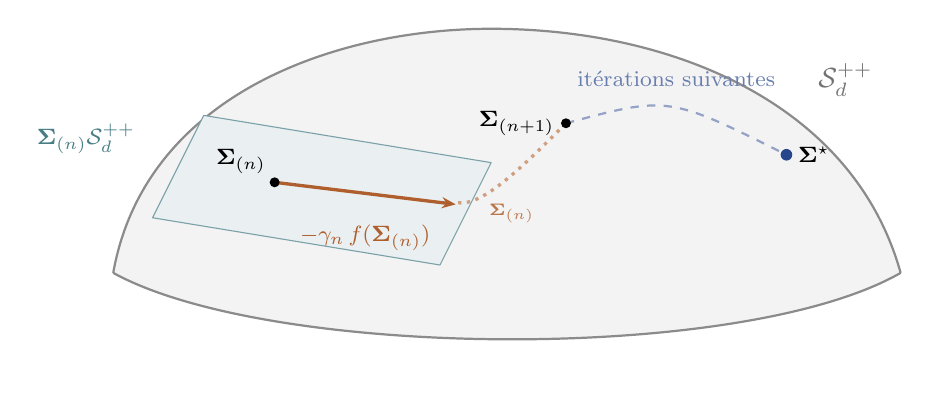
\begin{tikzpicture}[
    >={Stealth[length=5pt,width=4pt]},
    line join=round,
    font=\footnotesize,
  ]
  \definecolor{rmanifold}{RGB}{90,90,90}
  \definecolor{rtangent}{RGB}{50,110,120}
  \definecolor{rgeodesic}{RGB}{40,70,140}
  \definecolor{rvector}{RGB}{175,95,45}

  \coordinate (Sn)  at (-2.95,1.35);
  \coordinate (Sn1) at ( 0.75,2.10);
  \coordinate (Sst) at ( 3.55,1.70);

  % ---------------------------------------------------------------- variete
  \fill[rmanifold!7]
    (-5.0,0.2) .. controls (-4.6,2.45) and (-2.2,3.3) .. (-0.2,3.3)
    .. controls ( 2.1,3.3) and ( 4.4,2.35) .. ( 5.0,0.2)
    .. controls ( 3.0,-0.9) and (-3.0,-0.95) .. (-5.0,0.2) -- cycle;
  \draw[rmanifold!70, thick]
    (-5.0,0.2) .. controls (-4.6,2.45) and (-2.2,3.3) .. (-0.2,3.3)
    .. controls ( 2.1,3.3) and ( 4.4,2.35) .. ( 5.0,0.2);
  \draw[rmanifold!70, thick]
    (-5.0,0.2) .. controls (-3.0,-0.9) and (3.0,-0.95) .. (5.0,0.2);
  \node[rmanifold!85, font=\normalsize] at (4.30,2.65) {$\SPD{\Nvar}$};

  % ---------------------------------------------------- plan tangent en Sn
  \fill[rtangent!10, draw=rtangent!65]
    ($(Sn)+(-1.55,-0.45)$) -- ($(Sn)+(2.10,-1.05)$)
    -- ($(Sn)+(2.75,0.25)$) -- ($(Sn)+(-0.90,0.85)$) -- cycle;
  \node[rtangent!90, anchor=east] at ($(Sn)+(-1.65,0.55)$)
    {$\Tangent{\MCov_{(\iiter)}}{\SPD{\Nvar}}$};

  % -------------------------------------------------- direction de descente
  \draw[rvector, very thick, ->] (Sn) -- ($(Sn)+(2.30,-0.28)$);
  \node[rvector, anchor=north] at ($(Sn)+(1.15,-0.42)$)
    {$-\gamma_\iiter\,\Rgrad f(\MCov_{(\iiter)})$};

  % ---------------------------------------------------------- retraction
  \draw[rvector!60, dotted, very thick]
    ($(Sn)+(2.33,-0.26)$) .. controls (-0.30,1.05) and (0.20,1.55) .. (Sn1);
  \node[rvector!85, anchor=north west] at (-0.35,1.20)
    {$\Retr_{\MCov_{(\iiter)}}$};

  % ------------------------------------------------ suite des iteres et opt.
  \draw[rgeodesic!50, thick, dashed]
    (Sn1) .. controls (2.05,2.45) .. (Sst);
  \node[rgeodesic!70, anchor=south] at (2.15,2.44) {itérations suivantes};

  \fill (Sn) circle (1.8pt);
  \node[anchor=south east, inner sep=3pt] at (Sn) {$\MCov_{(\iiter)}$};
  \fill (Sn1) circle (1.8pt);
  \node[anchor=east, inner sep=4pt] at (Sn1) {$\MCov_{(\iiter+1)}$};
  \fill[rgeodesic] (Sst) circle (2.1pt);
  \node[anchor=west, inner sep=4pt] at (Sst) {$\MCov^{\opt}$};
\end{tikzpicture}

\end{document}
